% ===== 原文 pp.1--12：§1 引言 + §2 标题 + §2.1 + 2.2/2.2.1 标题（Lead）=====
% [原文 p.3]
\section{引言}

本讲义旨在介绍量子场论（QFT）中的\textbf{广义整体对称性}（generalized global symmetries）这一课题。
过去十年间，这一领域的研究活动极为密集；相关研究与高能物理（包括量子引力）以及理论凝聚态物理等广阔研究方向相联系。
这一热潮的主要来源是：人们有望以类似于利用整体对称性的方式，来利用这些广义对称性，从而探测 QFT 及相关课题中的各种物理现象。
整体对称性及其 't Hooft 反常在重整化群（RG）流下不变，因此可以用来探测超出微扰论标准工具所能及的强耦合物理。

% [原文 p.4]
与此相关的是：整体对称性的自发破缺提供了一个 Landau--Ginzburg 式的有力范式，用来理解相结构并在红外（IR）整理相图。
正如我们将要讨论的，所有这些在研究标准整体对称性时已熟悉的概念，同样适用于广义整体对称性的研究。

\para{相关文献。}
我们一开始就要指出：本讲义只介绍所谓的\textbf{可逆}（invertible）广义对称性，其中包括高阶形式对称性与高阶群对称性。
过去两年里，该领域的大部分近期努力集中在\textbf{不可逆}对称性的研究上。关于不可逆对称性这一主题的一组优秀入门讲义，读者可参考新近出现的文献 [1]。
对于没有该领域背景、又希望一直了解到该领域前沿的读者，我们建议把本讲义与文献 [1] 配对阅读。
我们也注意到新近的手稿 [2]，它面向高能唯象学家介绍广义整体对称性；我们的讲法与之互补，面向高能理论家。
文献 [3] 还给出了另一组更为入门的讲义。

\para{预备知识。}
本讲义面向中等或高年级研究生。物理预备知识包括对量子场论（含其非微扰方面）的深入理解。
读者应熟悉非阿贝尔规范理论、磁单极子、背景场形式、反常、自发对称性破缺与 Higgs 机制。
部分例子还假定读者具备一些超对称知识，但理解基本概念并不需要它。
数学预备知识包括对微分几何与代数拓扑的良好理解，达到高等量子场论与弦论课程中所用的水平。良好的群论基础也将极有帮助。

\para{本讲义的安排。}
本讲义组织如下：
\begin{itemize}[leftmargin=1.6em,itemsep=2pt,topsep=2pt]
\item 第 2 节把常用的整体对称性概念重新表述为拓扑算符，从而引入作为整体对称性推广的\textbf{高阶形式对称性}。
  文中讨论允许高阶形式对称性的许多量子场论例子，包括 Maxwell 理论与离散规范理论。
% [原文 p.5]
\item 第 3 节讨论一般 阿贝尔与非阿贝尔规范理论的\textbf{高阶形式对称性}。从较理论的视角看，本节可视为大量例子的汇集；
  从较实用的视角看，本节也可视为对规范理论中许多细微性质（在规范理论的初次介绍中往往未被强调）的描述。
\item 第 4 节讨论与高阶形式对称性相关的各种性质，它们构成了把这些对称性用于物理应用时的基本工具箱。
  内容包括 't Hooft 反常、对称性保护拓扑（SPT）相、这些对称性的规范化（gauging）与自发对称性破缺。
  我们还引入\textbf{对称性拓扑场论}（symmetry topological field theory，SymTFT）的概念。
\item 第 5 节介绍\textbf{高阶群对称性}。这些是新的对称结构，可以解释为由高阶形式对称性的「混合」（mixings）产生。
  我们讨论涉及连续与离散高阶形式对称性的各种高阶群对称性，并描述它们如何在各种规范理论中出现；
  不过我们不会深入其 't Hooft 反常、规范化与自发破缺等性质。到本文这一阶段，我们相信读者已有能力从所列参考文献中轻松补齐这些概念。
\item 第 6 节简要介绍在弦论给出的量子场论几何工程（geometric engineering）构造中研究高阶形式对称性，
  以及用全息（holographic）对偶研究高阶形式对称性。
\end{itemize}

% [Tutor Note: 本节（§1）为全文纲要，没有编号公式；原文在此未给出公理化定义，术语在 §2 起才逐步引入，
%   阅读时可将 §1 的六条纲要与 §2--§6 的标题对照：§2 高阶形式、§3 规范理论例子、§4 性质工具箱（反常/SPT/gauging/SSB/SymTFT）、
%   §5 高阶群、§6 弦论与全息。]

\section{高阶形式对称性导论}

本节旨在介绍 $p$-形式对称性。这类对称性推广了通常的整体对称性——在后者的语言中，它们被称为 0-形式对称性。
我们将遵循奠基性工作 [4]，但这并不是说该文首次讨论了此类思想。事实上，其中涉及的许多想法可追溯到
1980 年代末与 1990 年代初不同学派关于规范理论非微扰方面、离散规范理论、有理 CFT 与 Chern--Simons 理论的研究。
见 [5--24]（排名不分先后）作为这些工作的一个小样本。此外，文献 [25--52] 是 [4] 的先驱。

\subsection{0-形式对称性}

让我们先回顾众所周知的 0-形式对称性情形。描述这种对称性的标准方式，是引入一个幺正算符
\begin{equation}
    U(t)\,, \tag{2.1}
\end{equation}
% [原文 p.6]
它作用在时刻 $t$ 的 Hilbert 空间上，并与生成时间演化的 Hamiltonian 对易，即
\begin{equation}
    U(t)=U(t')\,,\qquad \forall\, t,t'\,. \tag{2.2}
\end{equation}
此外，$U(t)$ 作用在整个空间上，因为它作用在位于空间任意点的局域算符上。该作用通过共轭实现
\begin{equation}
    U(t)\,\cO(\vec{x},t)\,U^{-1}(t)=\cO'(\vec{x},t)\,, \tag{2.3}
\end{equation}
它把局域算符 $\cO(\vec{x},t)$ 变换为另一个局域算符 $\cO'(\vec{x},t)$。

文献 [4] 的关键洞见是：上述算符 $U(t)$ 的性质可以重新表述如下：

\begin{statementbox}{陈述 2.1：0-形式对称性是拓扑余维-1 算符}
一个 0-形式对称性就是一个既拓扑又可逆的余维-1 算符 $U$。
\end{statementbox}

让我们进一步展开这一陈述：

\para{沿一般余维-1 子流形的插入。}
余维-1 算符 $U$ 可以插在 $d$ 维时空内的任意余维-1 流形 $\Sigma_{d-1}$ 上（该流形可以是紧致的，也可以不是）。
插入后，该算符记为
\begin{equation}
    U(\Sigma_{d-1})\,. \tag{2.4}
\end{equation}
特别地，我们可以取
\begin{equation}
    \Sigma_{d-1}=\{\text{某一特定时刻 }t\text{ 的空间切片}\}\equiv\Sigma_t\,, \tag{2.5}
\end{equation}
此时所插入的算符可等同于上面讨论的作用在 Hilbert 空间上的幺正算符 $U(t)$
\begin{equation}
    U(\Sigma_t)\equiv U(t)\,. \tag{2.6}
\end{equation}

% [原文 p.7]
\begin{figure}[htbp]
\centering
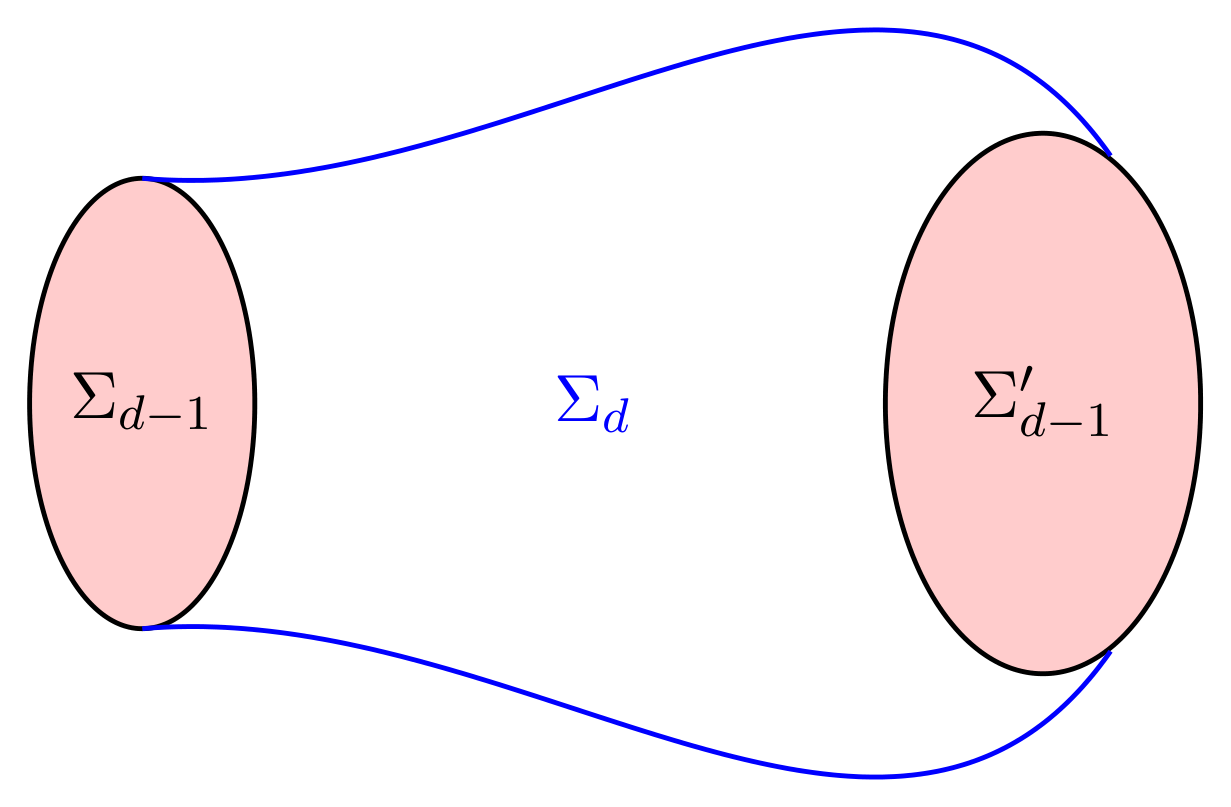
\includegraphics[width=0.78\textwidth]{fig1.png}
\figtitle{1}{两个 $(d-1)$ 维流形 $\Sigma_{d-1}$、$\Sigma'_{d-1}$，它们通过一次拓扑形变相联系。
$\Sigma_d$ 是一个 $d$ 维流形，其边界由 $\Sigma'_{d-1}$ 与 $\Sigma_{d-1}$ 的反向副本构成。
把拓扑算符 $U$ 沿 $\Sigma_{d-1}$ 插入，等价于把它沿 $\Sigma'_{d-1}$ 插入。}
\end{figure}

\begin{notebox}{关联函数中的算符}
注意，$U(\Sigma_{d-1})$ 最好解释为关联函数内部的余维-1 算符，而不是作用在 Hilbert 空间上的算符。
这是因为一旦选定了某个时间方向，子流形 $\Sigma_{d-1}$ 就不必是空间切片。
\end{notebox}

\para{拓扑性质。}
$U$ 是拓扑算符这一事实意味着
\begin{equation}
    U(\Sigma_{d-1})=U(\Sigma'_{d-1})\,, \tag{2.7}
\end{equation}
只要 $\Sigma'_{d-1}$ 是时空的余维-1 子流形、且可由 $\Sigma_{d-1}$ 经拓扑形变得到，即只要
\begin{equation}
    \Sigma'_{d-1}-\Sigma_{d-1}=\partial\Sigma_d\,, \tag{2.8}
\end{equation}
其中 $\partial\Sigma_d$ 是时空中某个 $d$ 维子流形 $\Sigma_d$ 的边界。见图 1。
余维-1 算符 $U(\Sigma_{d-1})$ 的这一拓扑性质 (2.7)，是幺正算符 $U(t)$ 与时间无关这一事实 (2.2) 的推广：
把
\begin{equation}
    \Sigma_{d-1}=\Sigma_t\,,\qquad \Sigma'_{d-1}=\Sigma_{t'}\,, \tag{2.9}
\end{equation}
代入 (2.7)，即可回收熟悉的陈述 (2.2)。

\para{可逆性质。}
$U$ 可逆这一事实意味着：存在另一个拓扑余维-1 算符 $U'$，使得
\begin{equation}
    U(\Sigma_{d-1})\,U'(\Sigma_{d-1})=1\,. \tag{2.10}
\end{equation}
也就是说，把 $U$ 与 $U'$ 同时插在同一个余维-1 子流形 $\Sigma_{d-1}$ 上，等价于在 $\Sigma_{d-1}$ 上什么都不插。
采用记号
\begin{equation}
    U'\equiv U^{-1}\,, \tag{2.11}
\end{equation}
% [原文 p.8]
则方程 (2.10) 变为
\begin{equation}
    U(\Sigma_{d-1})\,U^{-1}(\Sigma_{d-1})=1\,. \tag{2.12}
\end{equation}
对于作用在 Hilbert 空间上的算符 (2.6)，可逆性来自它们都是幺正的。

\para{对局域算符的作用。}
对局域算符的作用 (2.3)，可以用一般的算符 $U(\Sigma_{d-1})$ 表述为如下方程（在关联函数内部有效）
\begin{equation}
    U(\Sigma_{d-1})\,\cO(x)=\cO'(x)\,U(\Sigma'_{d-1})\,, \tag{2.13}
\end{equation}
其中
\begin{equation}
    x\equiv(\vec{x},t) \tag{2.14}
\end{equation}
是位于时空子流形 $\Sigma_d$ 内的一点，而 $\Sigma_d$ 按 (2.8) 联系 $\Sigma_{d-1}$ 与 $\Sigma'_{d-1}$。
给定方程 (2.13)，我们说 0-形式对称性 $U$ 作用在局域算符 $\cO(x)$ 上，把它变成局域算符 $\cO'(x)$。
把 (2.9) 代入 (2.13) 并取极限
\begin{equation}
    \Delta t=t'-t\to0\,, \tag{2.15}
\end{equation}
即可回收方程 (2.3)。

\para{通过环绕实现的作用。}
描述作用 (2.13) 的另一种等价方式是
\begin{equation}
    U(S^{d-1})\,\cO(x)=\cO'(x)\,, \tag{2.16}
\end{equation}
其中左边把算符 $U$ 插在一个环绕时空点 $x$ 的 $(d-1)$ 维球面 $S^{d-1}$ 上，如图 2 所示。
作用的这一表示 (2.16) 可如 图 2 所述由 (2.13) 得到。

% [原文 p.9]
\begin{figure}[htbp]
\centering
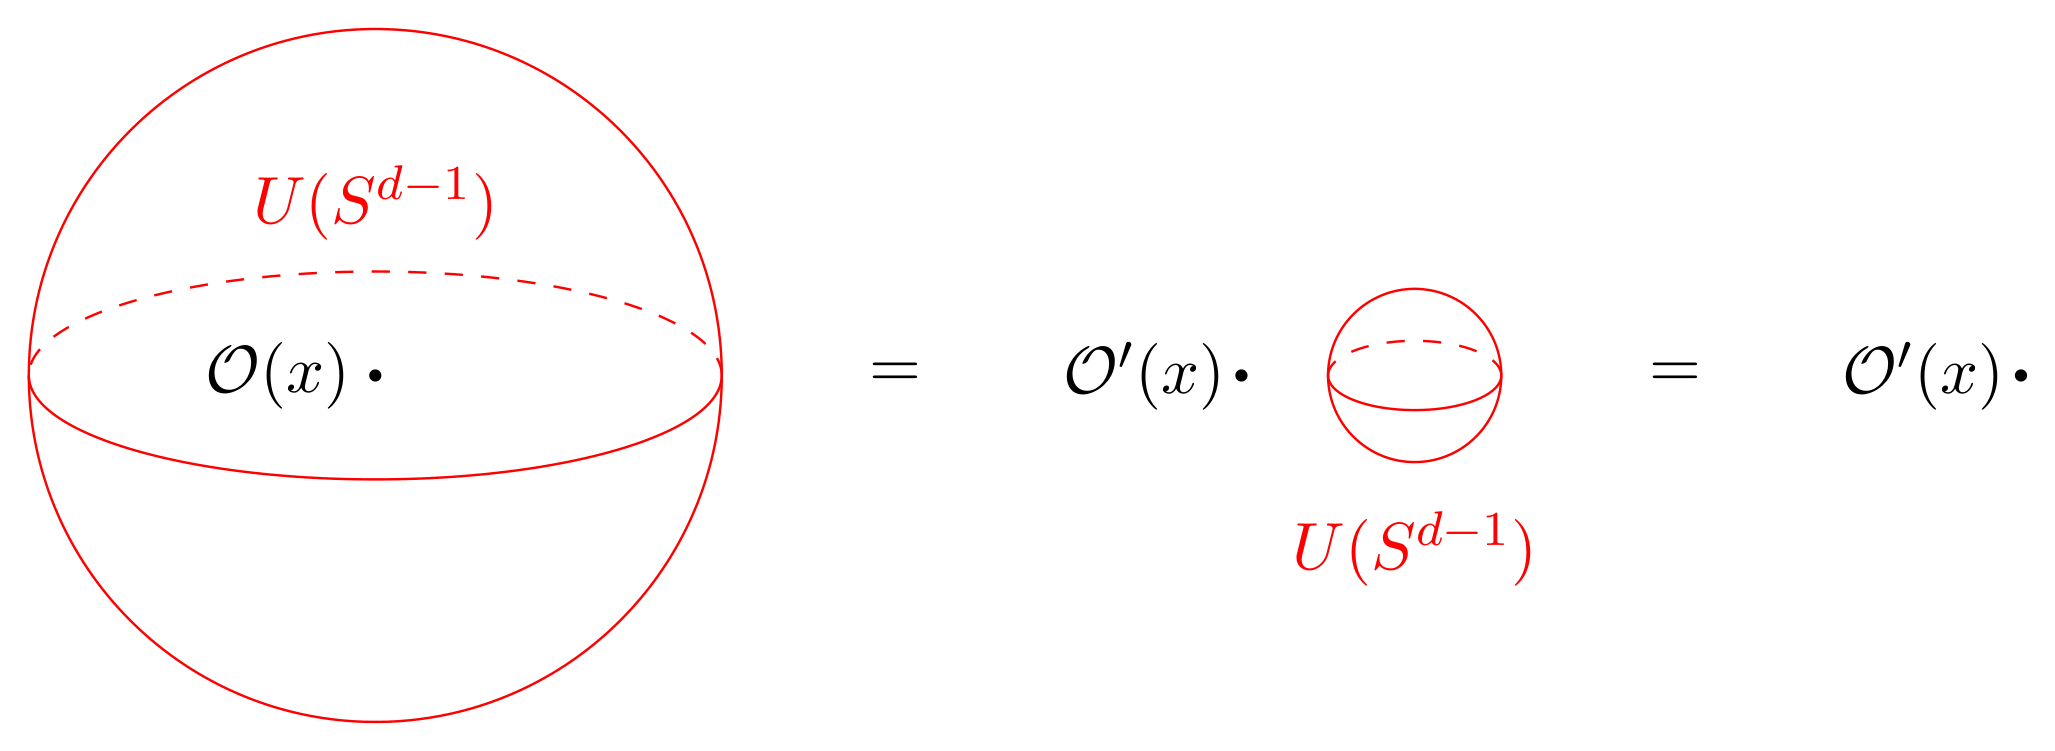
\includegraphics[width=0.92\textwidth]{fig2.png}
\figtitle{2}{左：把拓扑算符 $U$ 插在环绕局域算符 $\cO$ 所在点 $x$ 的球面 $S^{d-1}$ 上。
中：对 $U(S^{d-1})$ 作拓扑形变，使其不再环绕 $x$；由 (2.13)，这一过程把位于 $x$ 的局域算符改为 $\cO'$。
右：此时 $S^{d-1}$ 是某个 $d$ 维球的边界，故可以把 $U(S^{d-1})$ 缩掉。}
\end{figure}

\para{0-形式对称群。}
一般地，0-形式对称性组合成一个（可能非阿贝尔的）0-形式对称群
\begin{equation}
    G^{(0)}\,. \tag{2.17}
\end{equation}
这意味着我们有拓扑余维-1 算符
\begin{equation}
    U_g\,,\qquad \forall\, g\in G^{(0)}\,, \tag{2.18}
\end{equation}
它们由群 $G^{(0)}$ 的元素参数化。群的乘法描述这些算符的复合
\begin{equation}
    U_g(\Sigma_{d-1})\,U_{g'}(\Sigma_{d-1})=U_{gg'}(\Sigma_{d-1})\,, \tag{2.19}
\end{equation}
它常被记作融合规则（fusion rule）
\begin{equation}
    U_g\otimes U_{g'}=U_{gg'}\,. \tag{2.20}
\end{equation}
若把 $\Sigma_{d-1}$ 限制为时间切片，从而把 $U$ 限制为作用在 Hilbert 空间上的幺正算符，(2.19) 变为
\begin{equation}
    U_g(t)\,U_{g'}(t)=U_{gg'}(t)\,, \tag{2.21}
\end{equation}
这意味着 Hilbert 空间构成 0-形式对称群 $G^{(0)}$ 的一个表示。
类似地，（某时空点 $x$ 处的）局域算符构成的向量空间也构成 $G^{(0)}$ 的一个表示。为看出这一点，
利用算符 $U_g$ 对局域算符作用的表示式 (2.16)
\begin{equation}
    U_g\!\left(S^{d-1}\right)\cO(x)=g\cdot\cO(x)\,. \tag{2.22}
\end{equation}

% [原文 p.10]
利用 (2.19) 取 $\Sigma_{d-1}=S^{d-1}$，我们得到
\begin{equation}
    g\cdot\big(g'\cdot\cO(x)\big)=(gg')\cdot\cO(x)\,. \tag{2.23}
\end{equation}
见 图 3。

\begin{figure}[htbp]
\centering
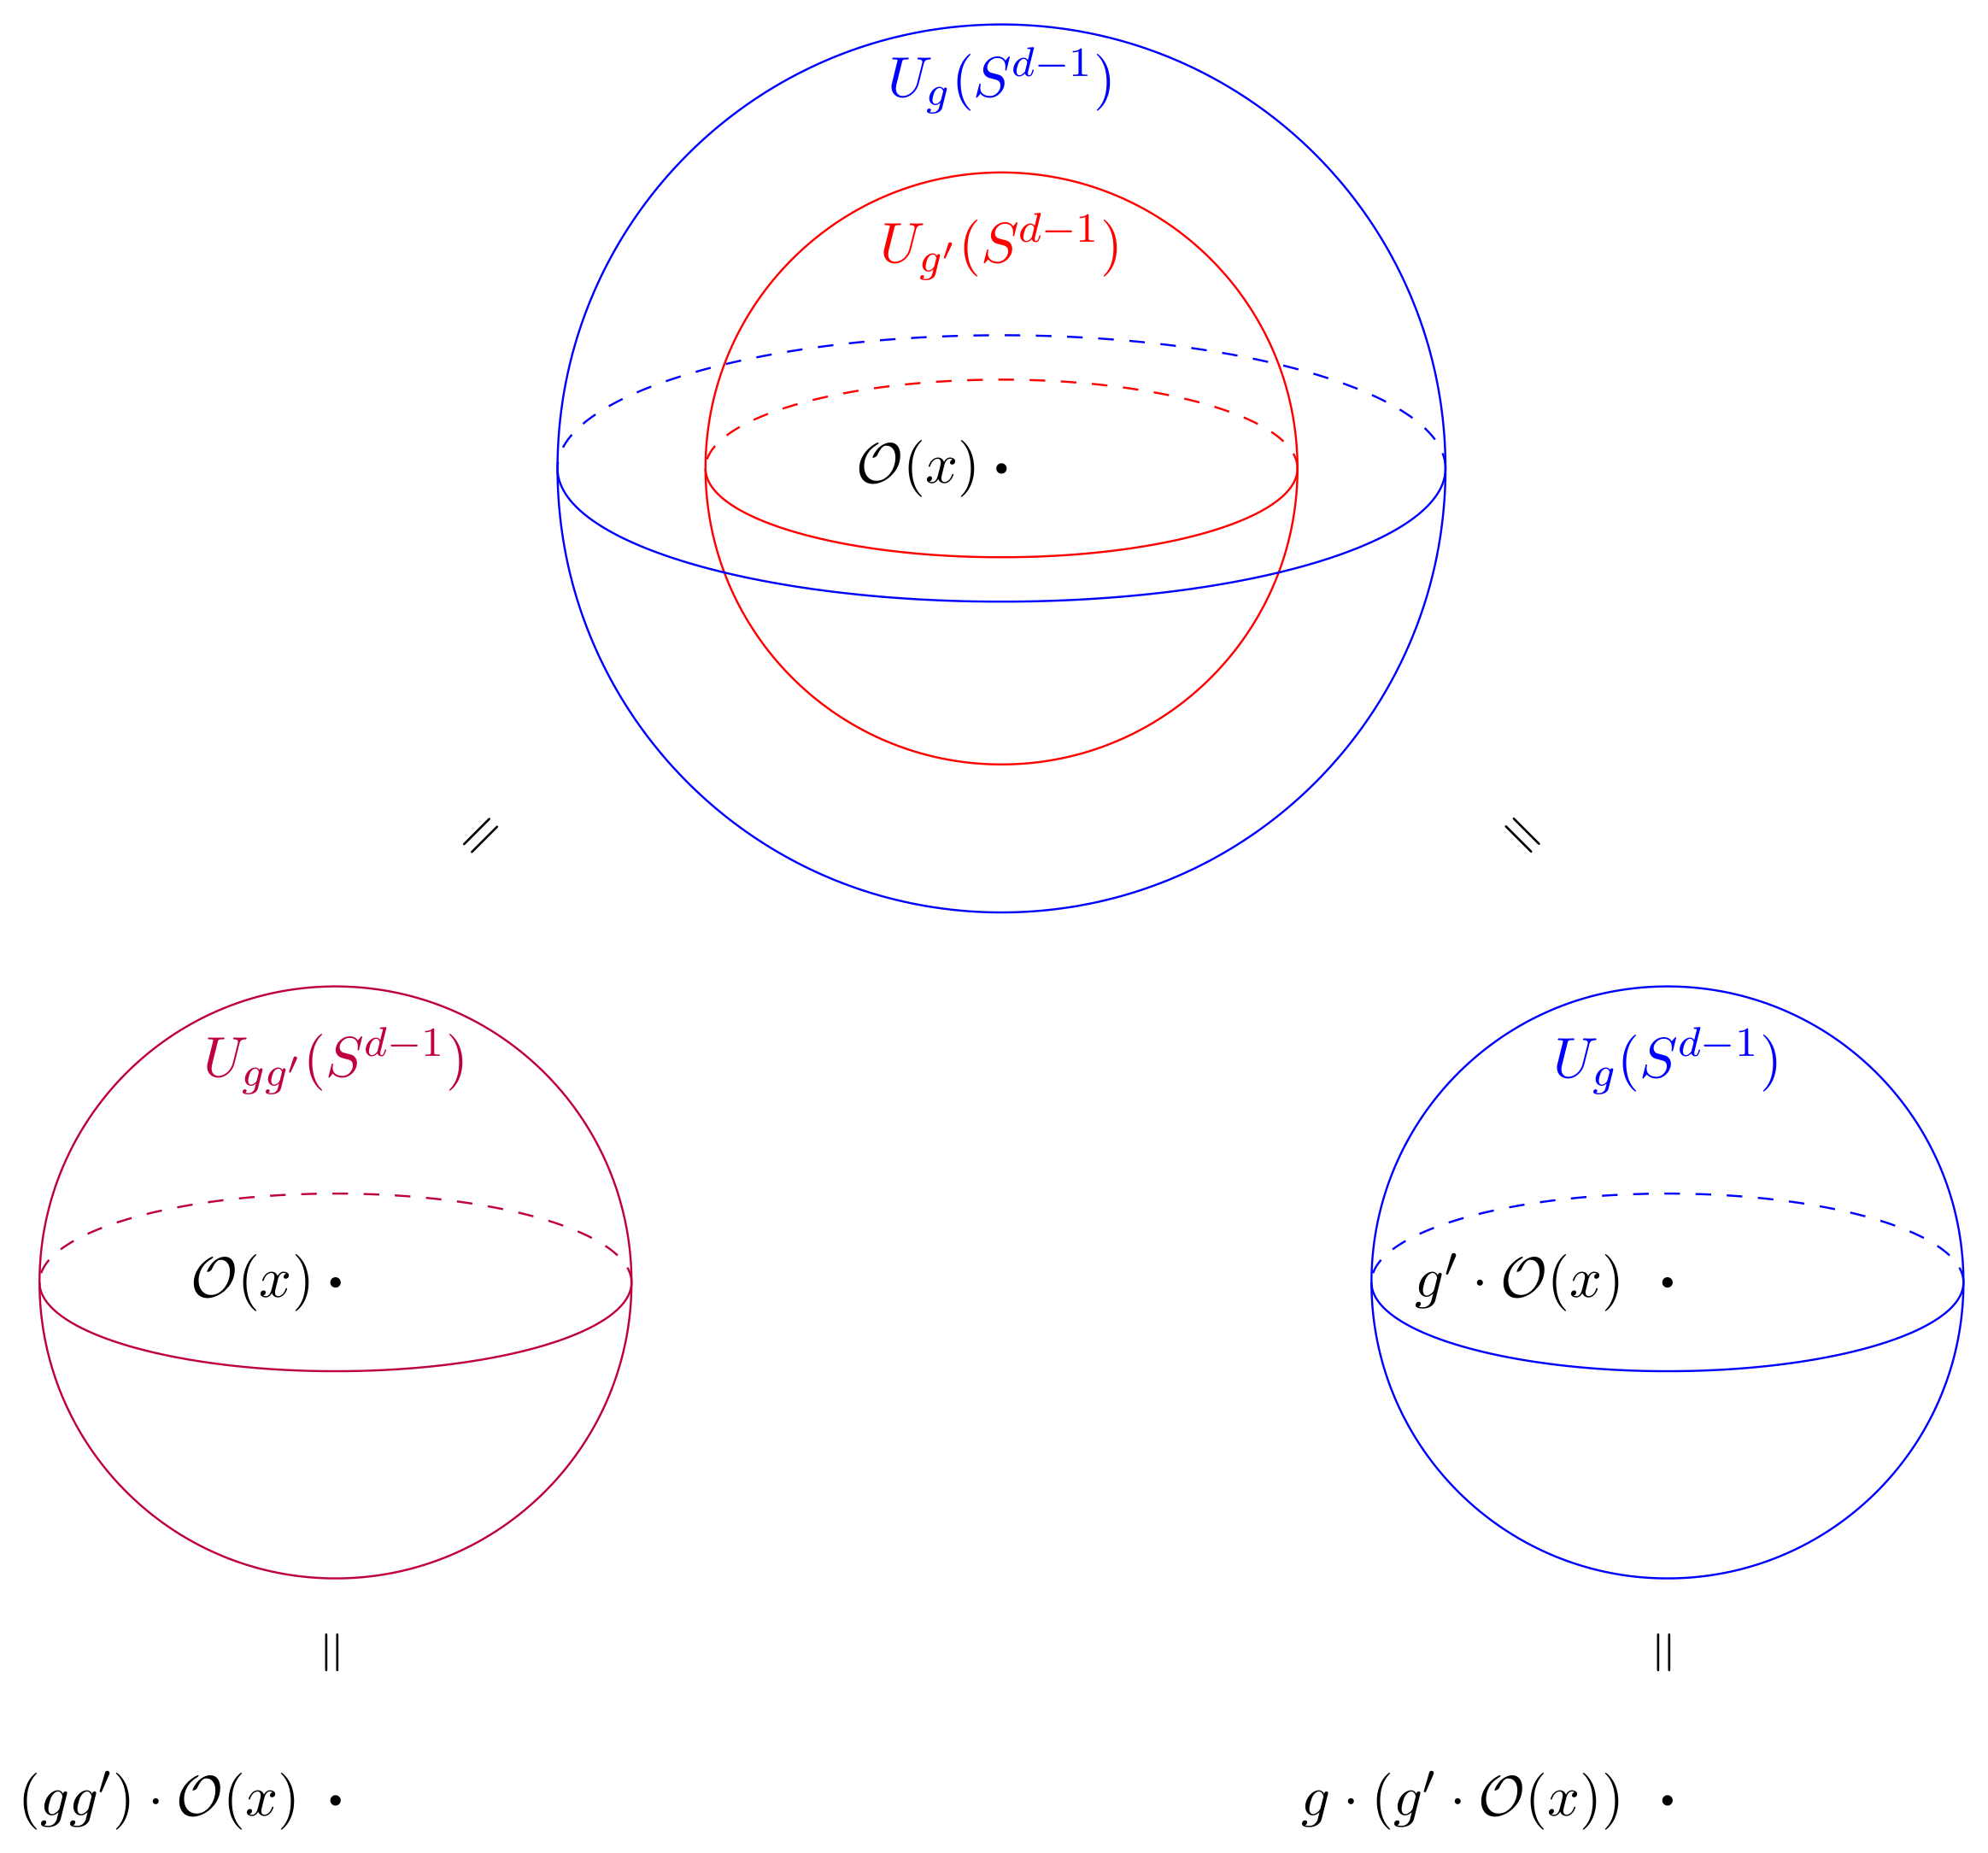
\includegraphics[width=0.92\textwidth]{fig3.png}
\figtitle{3}{从最上方的构型出发，我们既可以走左边的路径：先融合拓扑算符，再作用于局域算符；
也可以走右边的路径：依次作用于局域算符 $\cO$。两条路径必须给出相同结果，于是得到方程 (2.23)。}
\end{figure}

\begin{examplebox}{例 2.1：$\U(1)$ 0-形式对称性}
考虑
\begin{equation}
    G^{(0)}=U(1)\,, \tag{2.24}
\end{equation}
这个例子很好地说明了上述所有概念。
这种对称性联系着一个 Noether 流\footnote{最近文献 [53] 指出了 Noether 定理有效性的若干反例。}，
它是一个满足连续性方程的局域算符 $j^\mu(x)$
\begin{equation}
    \partial_\mu j^\mu=0\,. \tag{2.25}
\end{equation}
由此通常定义电荷算符
\begin{equation}
    Q(t)=\int\dd^{d-1}\vec{x}\ j^0(\vec{x},t)\,, \tag{2.26}
\end{equation}
它满足
\begin{equation}
    \frac{\dd Q}{\dd t}=0\,, \tag{2.27}
\end{equation}
这是 (2.25) 的推论。在 Hilbert 空间上实现 $\U(1)$ 整体对称性的幺正算符 $U_g(t)$（$g\in \U(1)$）构造为
\begin{equation}
    U_g(t)=\exp\big(\ii\alpha Q(t)\big)\,,\qquad g=\ee^{\ii\alpha}\in U(1)\,, \tag{2.28}
\end{equation}
它们满足
\begin{equation}
    U_g(t')=U_g(t)\,, \tag{2.29}
\end{equation}
这是 (2.27) 的推论。
% [Tutor Note: 例 2.1 是全文反复套用的模板：0-形式对称性 ↔ Noether 流。(2.30) 中的 $(d-1)$-形式 $j^{d-1}$ 正是 $j^\mu$ 的 Hodge 对偶，
%   $j^{d-1}_{\mu_1\cdots\mu_{d-1}}=\epsilon_{\mu_1\cdots\mu_{d-1}\mu_d}j^{\mu_d}$，因此 (2.32) 的闭性 $\dd j^{d-1}=0$ 与 (2.25) 的守恒律 $\partial_\mu j^\mu=0$ 等价；
%   核对方法：在 $d=4$ 时 $j^{3}=\epsilon_{\mu\nu\rho\sigma}j^\sigma$ 的微分给出 $\partial_\mu j^\mu$，这正是后文把高阶形式对称性统一表述为「拓扑算符」的来源。]
现在描述相关的拓扑余维-1 算符 $U_g$。在时空的任意子流形 $\Sigma_{d-1}$ 上的插入可写为
\begin{equation}
    U_g(\Sigma_{d-1})=\exp\left(\ii\alpha\int_{\Sigma_{d-1}}j^{d-1}\right), \tag{2.30}
\end{equation}
其中 $j^{d-1}$ 是时空上的一个 $(d-1)$-形式，其指标形式为
\begin{equation}
    j^{d-1}_{\mu_1\mu_2\cdots\mu_{d-1}}=\epsilon_{\mu_1\mu_2\cdots\mu_{d-1}\mu_d}\,j^{\mu_d}\,, \tag{2.31}
\end{equation}
其中 $\epsilon_{\mu_1\mu_2\cdots\mu_{d-1}\mu_d}$ 是完全反对称的 Levi-Civita 张量。这个 $(d-1)$-形式是闭的
\begin{equation}
    \dd j^{d-1}=0\,, \tag{2.32}
\end{equation}
% [原文 p.11]
作为 (2.25) 的推论，这蕴含如下拓扑性质
\begin{align}
    U_g(\Sigma'_{d-1}) &= U_g(\Sigma_{d-1})\times\exp\left(\ii\alpha\int_{\Sigma'_{d-1}-\Sigma_{d-1}=\partial\Sigma_d}j^{d-1}\right), \notag\\
    &= U_g(\Sigma_{d-1})\times\exp\left(\ii\alpha\int_{\Sigma_d}\dd j^{d-1}\right), \tag{2.33}\\
    &= U_g(\Sigma_{d-1})\,. \notag
\end{align}
% [原文 p.12]
在存在荷为
\begin{equation}
    q\in\Z \tag{2.34}
\end{equation}
的局域算符 $\cO(x)$ 时（在 $\U(1)$ 下），连续性方程修改为
\begin{equation}
    \cO(x)\,\partial_\mu j^\mu(x')=q\,\delta(x-x')\,\cO(x)\,, \tag{2.35}
\end{equation}
或用 $(d-1)$-形式写为
\begin{equation}
    \cO(x)\,\dd j^{d-1}=q\,\delta^d(x)\,\cO(x)\,, \tag{2.36}
\end{equation}
其中 $\delta^d(x)$ 是 $\delta(x-x')$ 的 $d$-形式 Poincar\'e 对偶。利用它，我们可以显式计算作用 (2.16) 为
\begin{align}
    U_g\!\left(S^{d-1}\right)\cO(x) &= \exp\left(\ii\alpha\int_{S^{d-1}}j^{d-1}\right)\cO(x)\,, \notag\\
    &= \exp\left(\ii\alpha\int_{D^d}\dd j^{d-1}\right)\cO(x)\,, \tag{2.37}\\
    &= \exp\left(\ii\alpha\int_{D^d}q\,\delta^d(x)\right)\cO(x)\,, \notag\\
    &= \exp(\ii q\alpha)\,\cO(x)\,. \notag
\end{align}
其中 $D^d$ 是包含点 $x$、边界为 $S^{d-1}$ 的 $d$ 维圆盘。
\end{examplebox}

\subsection{高阶形式对称性}

\subsubsection{一般性质}

% [原文 p.12]
高阶形式对称性的推广，是通过推广陈述 2.1 中的余维来实现的。

\begin{definitionbox}{定义 2.1：$p$-形式对称性}
一个 $p$-形式对称性就是一个既拓扑又可逆的余维-$(p+1)$ 算符 $U$。
\end{definitionbox}

我们可以通过与陈述 2.1 之后的讨论密切类比，来进一步展开上述定义。
% ===== c01 结束：下一句（p.13 首行「沿一般余维-(p+1) 子流形的插入。」）由 tr-01 续写 =====
